% Native editable composition from verified, unchanged IDE images.
\begin{figure}[htbp]
\centering
\sbox0{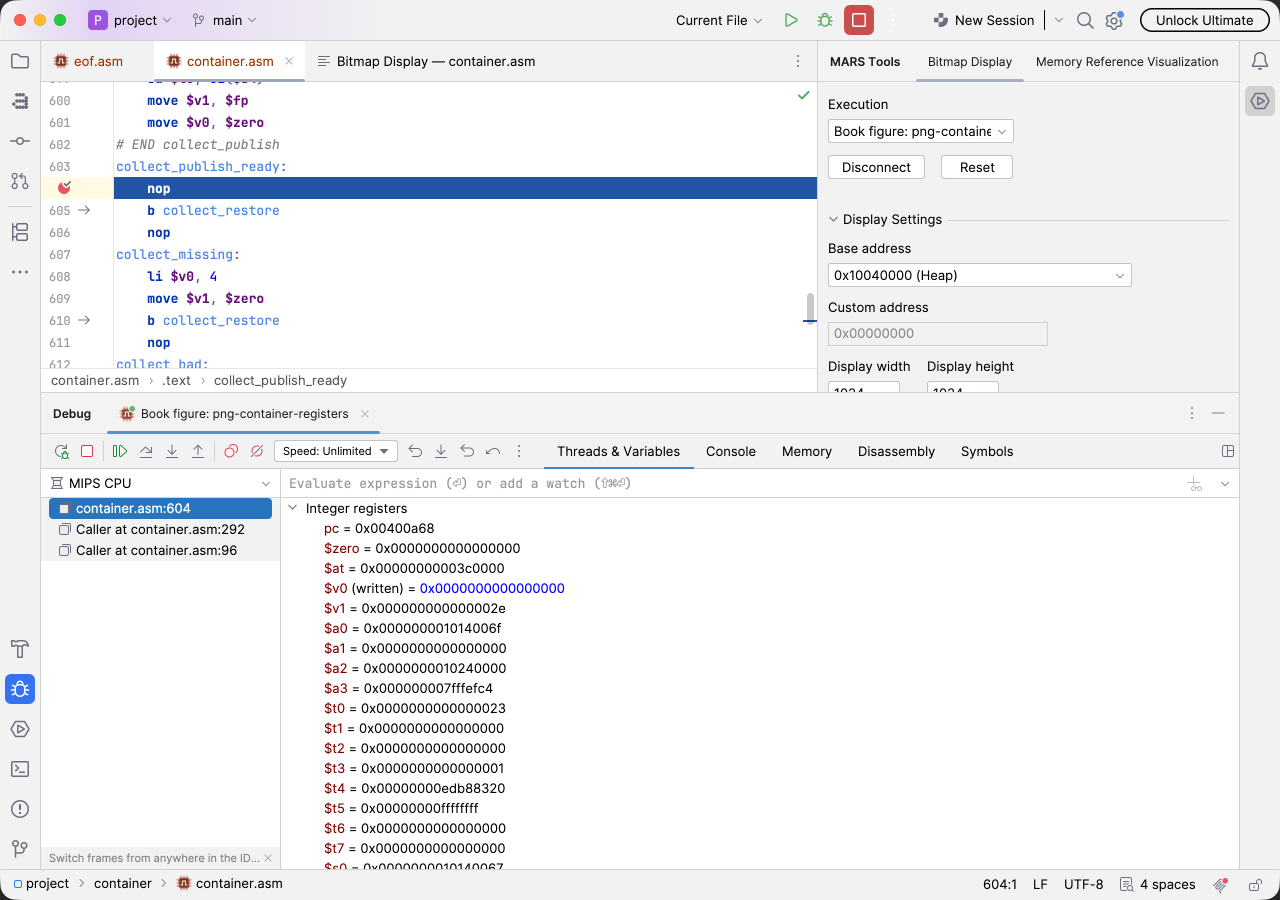
\includegraphics[artifact]{book/captures/033-png/png-container-fields/registers.png}}
\sbox2{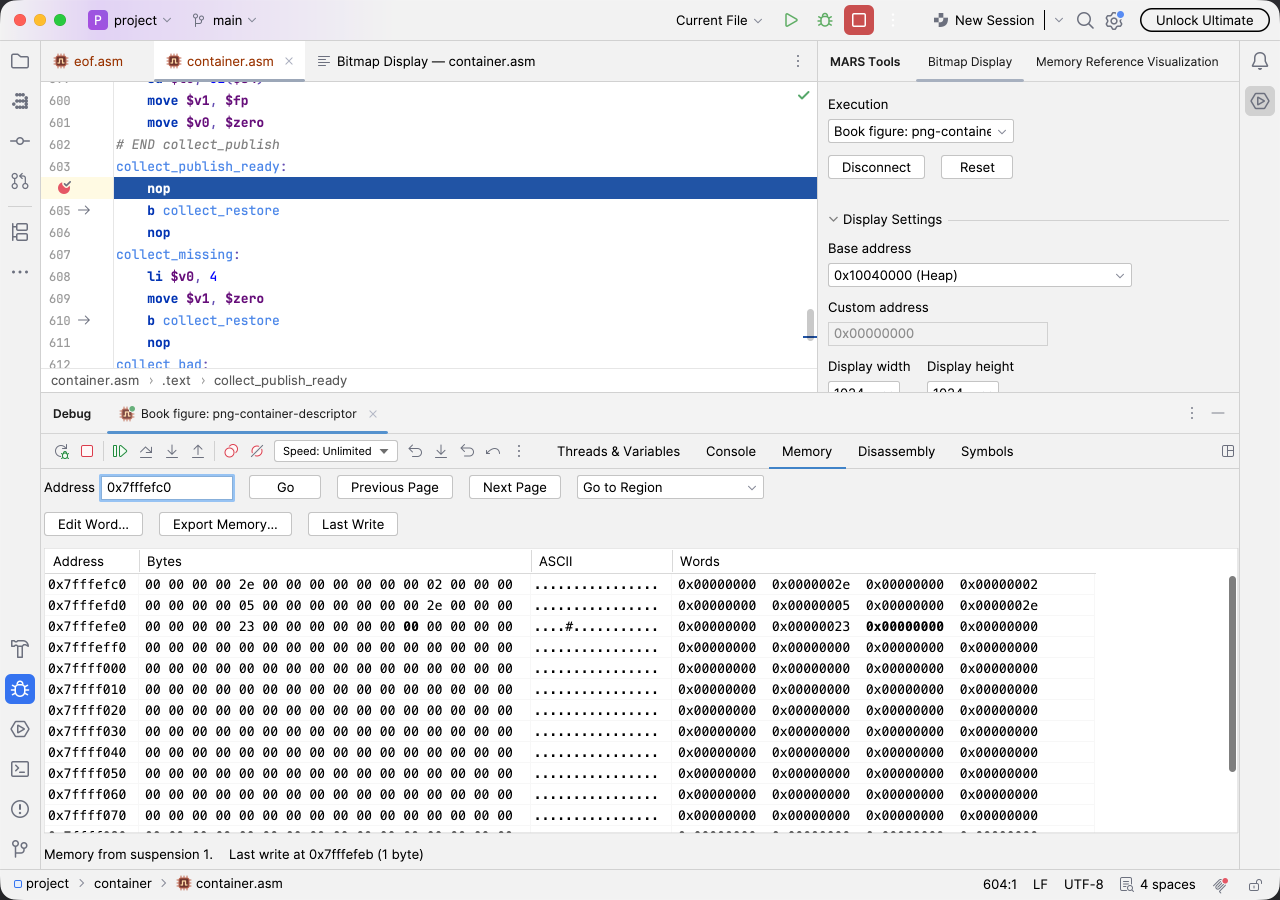
\includegraphics[artifact]{book/captures/033-png/png-container-fields/descriptor.png}}
\edef\MARScontainersourceLeft{\the\dimexpr0.036718750\wd0\relax}
\edef\MARScontainersourceBottom{\the\dimexpr0.774444444\ht0\relax}
\edef\MARScontainersourceRight{\the\dimexpr0.611718750\wd0\relax}
\edef\MARScontainersourceTop{\the\dimexpr0.170000000\ht0\relax}
\edef\MARScontainerdescriptorLeft{\the\dimexpr0.520312500\wd2\relax}
\edef\MARScontainerdescriptorBottom{\the\dimexpr0.288888889\ht2\relax}
\edef\MARScontainerdescriptorRight{\the\dimexpr0.139843750\wd2\relax}
\edef\MARScontainerdescriptorTop{\the\dimexpr0.634444444\ht2\relax}
\edef\MARScontainerreturnsLeft{\the\dimexpr0.246093750\wd0\relax}
\edef\MARScontainerreturnsBottom{\the\dimexpr0.310000000\ht0\relax}
\edef\MARScontainerreturnsRight{\the\dimexpr0.553125000\wd0\relax}
\edef\MARScontainerreturnsTop{\the\dimexpr0.638888889\ht0\relax}
\begin{tikzpicture}[alt={Three annotated IDE details at collect_publish_ready before its nop. The first 32-bit word precedes the descriptor. Starting at the second word, little-endian low/high pairs cross table-row boundaries and show capacity 46, width 2, height 5, joined zlib count 46 and predicted inflated count 35. Registers show success v0 zero and v1 46. Inflation and image publication have not run.}]
\node[anchor=north west,inner sep=0,font=\small\bfseries] (source-title) at (6mm,0) {Collector publication checkpoint};
\node[anchor=north west,inner sep=0] (source) at ([yshift=-1mm]source-title.south west) {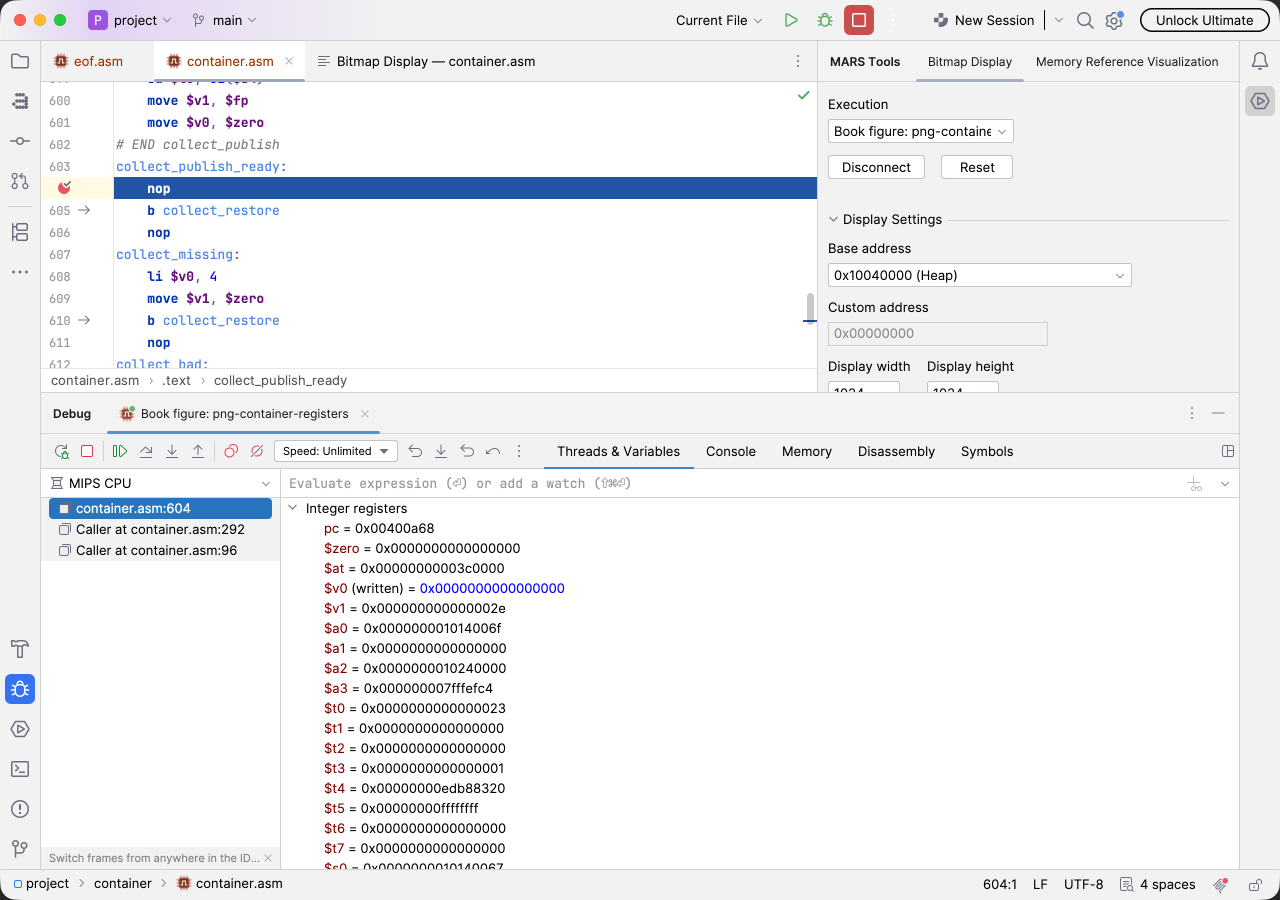
\includegraphics[width=0.7\linewidth,artifact,trim={\MARScontainersourceLeft{} \MARScontainersourceBottom{} \MARScontainersourceRight{} \MARScontainersourceTop{}},clip]{book/captures/033-png/png-container-fields/registers.png}};
\begin{scope}[shift={(source.south west)},x={($(source.south east)-(source.south west)$)},y={($(source.north west)-(source.south west)$)}]
\draw[black,line width=0.7pt] (0.153333333,0.080000000) rectangle (0.273333333,0.520000000);
\node[draw=black,fill=white,circle,inner sep=1.5pt,font=\footnotesize] at ($(0.153333333,0.520000000)+(-3mm,0)$) {1};
\end{scope}
\node[anchor=north west,inner sep=0,font=\small\bfseries] (descriptor-title) at ([yshift=-2mm]source.south west) {Capacity and four published doublewords};
\node[anchor=north west,inner sep=0] (descriptor) at ([yshift=-1mm]descriptor-title.south west) {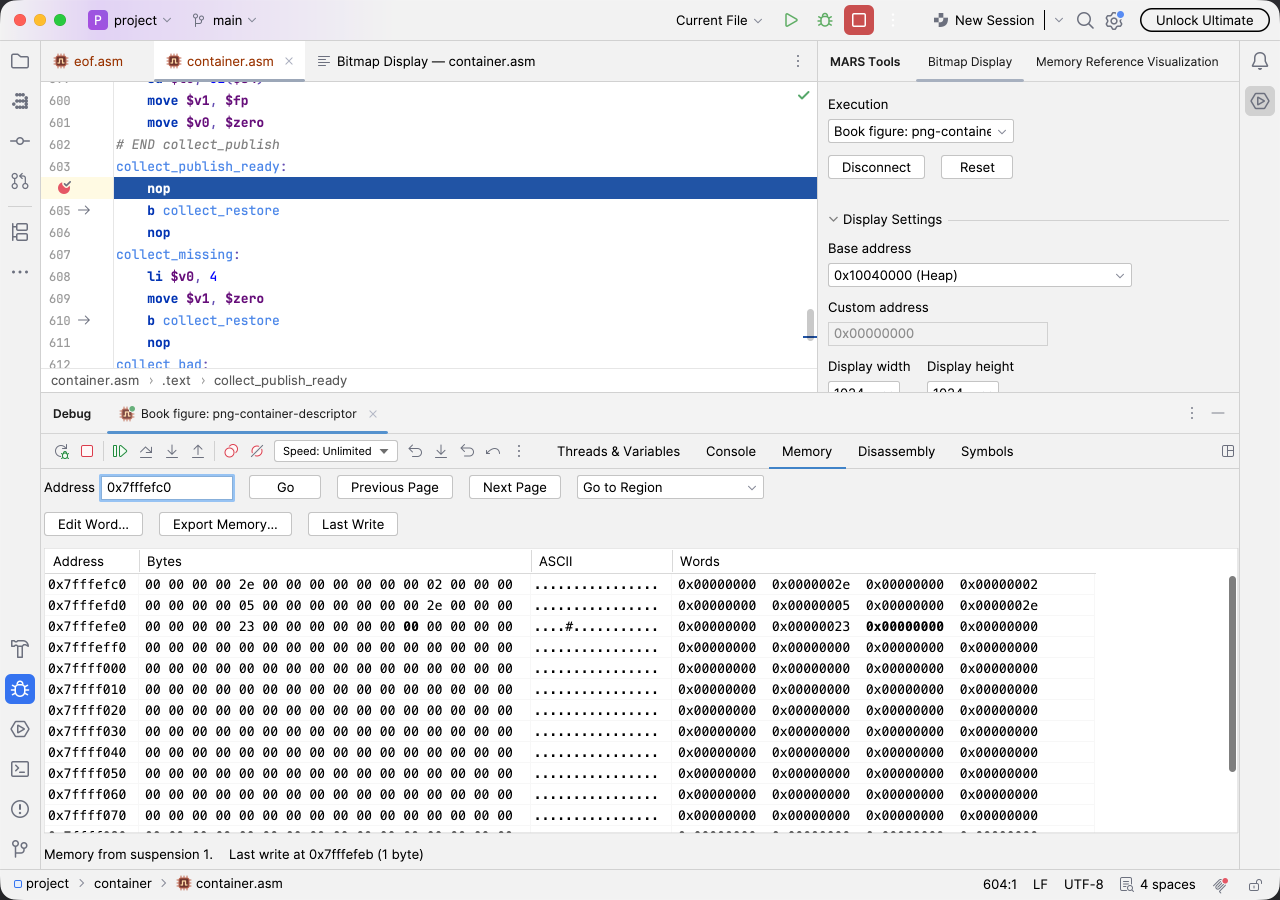
\includegraphics[width=0.84\linewidth,artifact,trim={\MARScontainerdescriptorLeft{} \MARScontainerdescriptorBottom{} \MARScontainerdescriptorRight{} \MARScontainerdescriptorTop{}},clip]{book/captures/033-png/png-container-fields/descriptor.png}};
\begin{scope}[shift={(descriptor.south west)},x={($(descriptor.south east)-(descriptor.south west)$)},y={($(descriptor.north west)-(descriptor.south west)$)}]
\draw[black,line width=0.7pt] (0.013793103,0.043478261) rectangle (0.986206897,0.956521739);
\node[draw=black,fill=white,circle,inner sep=1.5pt,font=\footnotesize] at ($(0.013793103,0.956521739)+(-3mm,0)$) {2};
\end{scope}
\node[anchor=north west,inner sep=0,font=\small\bfseries] (returns-title) at ([yshift=-2mm]descriptor.south west) {Success and joined zlib count};
\node[anchor=north west,inner sep=0] (returns) at ([yshift=-1mm]returns-title.south west) {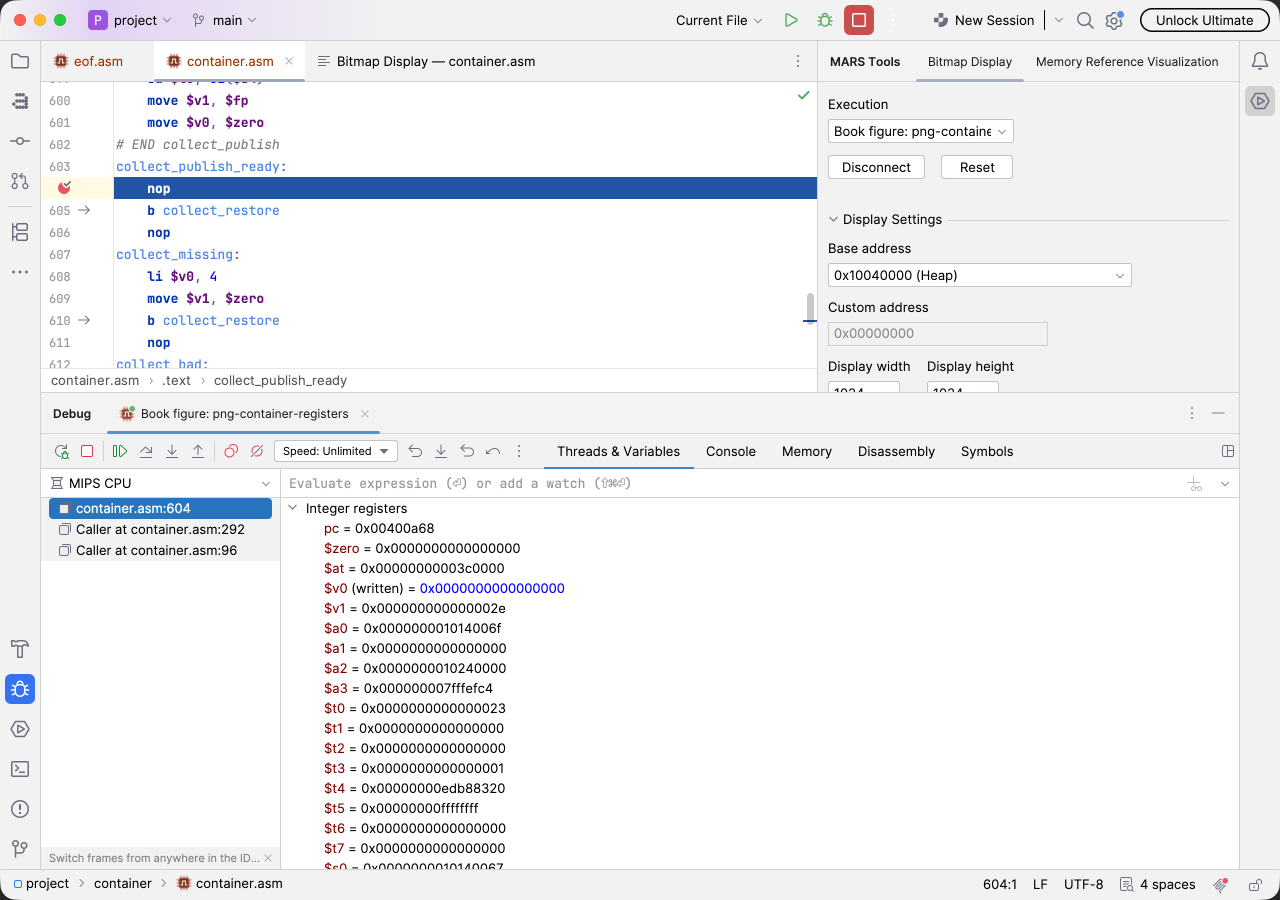
\includegraphics[width=0.5\linewidth,artifact,trim={\MARScontainerreturnsLeft{} \MARScontainerreturnsBottom{} \MARScontainerreturnsRight{} \MARScontainerreturnsTop{}},clip]{book/captures/033-png/png-container-fields/registers.png}};
\begin{scope}[shift={(returns.south west)},x={($(returns.south east)-(returns.south west)$)},y={($(returns.north west)-(returns.south west)$)}]
\draw[black,line width=0.7pt] (0.023346304,0.065217391) rectangle (0.976653696,0.934782609);
\node[draw=black,fill=white,circle,inner sep=1.5pt,font=\footnotesize] at ($(0.023346304,0.934782609)+(-3mm,0)$) {3};
\end{scope}
\end{tikzpicture}
\par\smallskip
\begin{minipage}{\linewidth}
\small
\begin{enumerate}
\item The container collector has completed its checks and stores. The checkpoint \texttt{nop} is next; no inflation or pixel publication has occurred.
\item The first word precedes the descriptor. Start at the second word and read low/high pairs across line breaks: capacity \texttt{0x2e}=46, width two, height five, joined count \texttt{0x2e}=46 and predicted inflated count \texttt{0x23}=35. The final word lies after the descriptor.
\item \texttt{\$v0}=0 and \texttt{\$v1}=46. The count includes zlib bytes; it is neither an RGB byte count nor a decoded framebuffer size.
\end{enumerate}
\end{minipage}
\caption{Accepted PNG container fields before inflation. Two Debug launches inspect the same publication checkpoint.}
\label{fig:png-container-fields}
\end{figure}
